\section{Demostración del Algortimo}

El algortimo desarrollado anteriormente nos afirma que nos va a dar la solución optima,
osea que Sophia gana todas las partidas de su nuevo juego, no importa el orden de los valores
de las monedas, dejando a Mateo como el perdedor tanto de cada ronda como del juego en si.

\vskip0.5cm

A continuación, se detallará el paso a paso de la demostración que hemos realizado para afirmar la teoria:

\vskip0.5cm

{\large{Sophie siempre ganas las partidas, por lo tanto también el juego}} 
\vskip0.5cm
Utilizamos el método por inducción:
\vskip0.5cm

Siendo $n$ la cantidad de monedas:
\vskip0.5cm

Si $n=1$ 

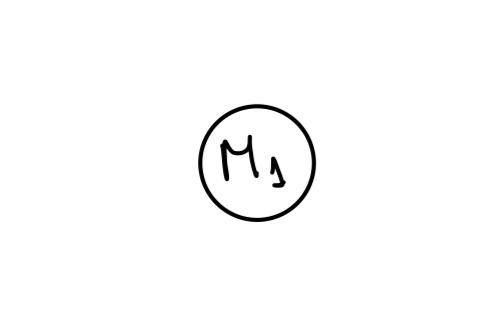
\includegraphics[width=6.5cm, height=4cm]{images/IMG_1625.jpg}


$valorSofiaMonedas=M_{1}$

$valorMateoMonedas=0$

Gana Sofia ya que siempre el primer turno es para ella, y solo hay una moneda.

\vskip1cm

Si $n=2$

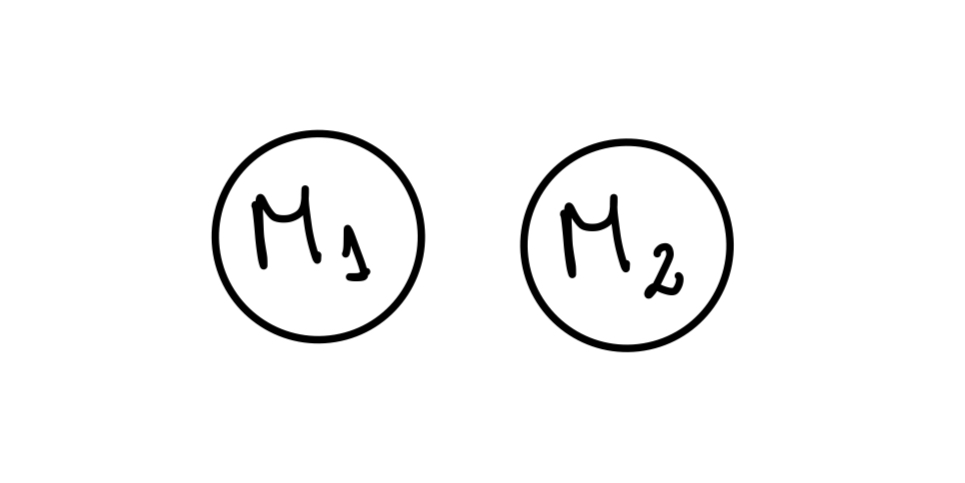
\includegraphics[width=6cm, height=3cm]{images/IMG_1626.jpg}

Siendo, $M_{1}>M_{2}$ : 


$valorSofiaMonedas=M_{1}$

$valorMateoMonedas=M_{2}$

Al empezar sofía, ella agarra la moneda más grande y gana
\vskip1cm
Si $n=3$

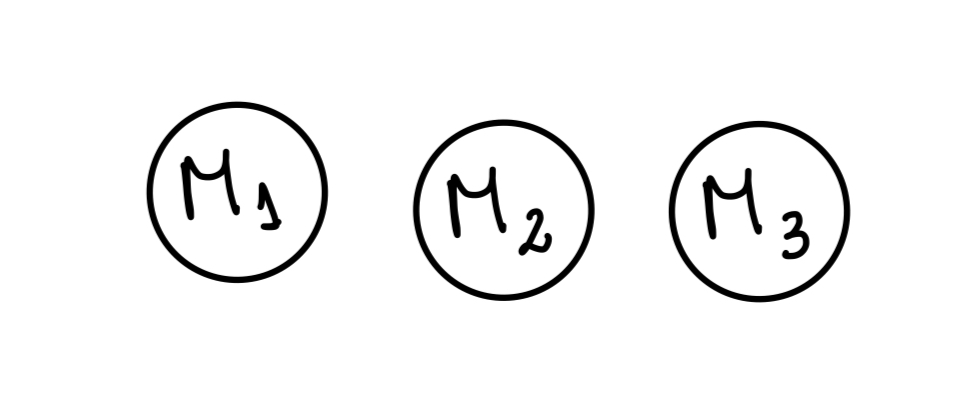
\includegraphics[width=6.5cm, height=3cm]{images/IMG_1627.jpg}

Siendo, $M_{1}<M_{2}<M_{3}$ : 


$valorSophiaMonedas=M_{3}+M_{2}$

$valorMateoMonedas=M_{1}$

Sophia agarra $M_{3}$ al ser el más grande, Mateo agarra (en realidad lo elige Sofía) el $M_{1}$ que es el valor
más pequeño, y por último Sophia agarra la moneda $M_{2}$ que es la última que quedaba. 
Sophia gana al tener las monedas de mayor valor.

\vskip1cm
Si $n=4$

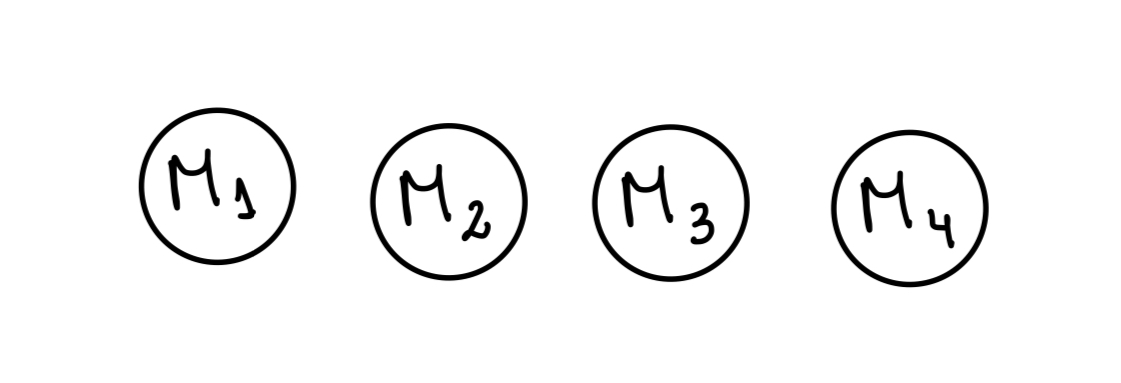
\includegraphics[width=8.5cm, height=3.5cm]{images/IMG_1628.jpg}

Siendo, $M_{4}<M_{3}<M_{1}<M_{2}$ : 

$valorSofiaMonedas=M_{1}+M_{2}$

$valorMateoMonedas=M_{4}+M_{3}$

Sofía agarra $M_{1}$ al ser la mas grande en comparación a $M_{4}$; Mateo agarra la moneda $M_{4}$ al ser la mas 
pequeña entre $M_{4}$ y $M_{2}$; Sofá agarra $M_{2}$ y por último por descarte Mateo se queda con la moneda $M_{3}$.
Gana Sofía por tener el mayor valor de monedas.

\vskip1cm
Si $n=k$

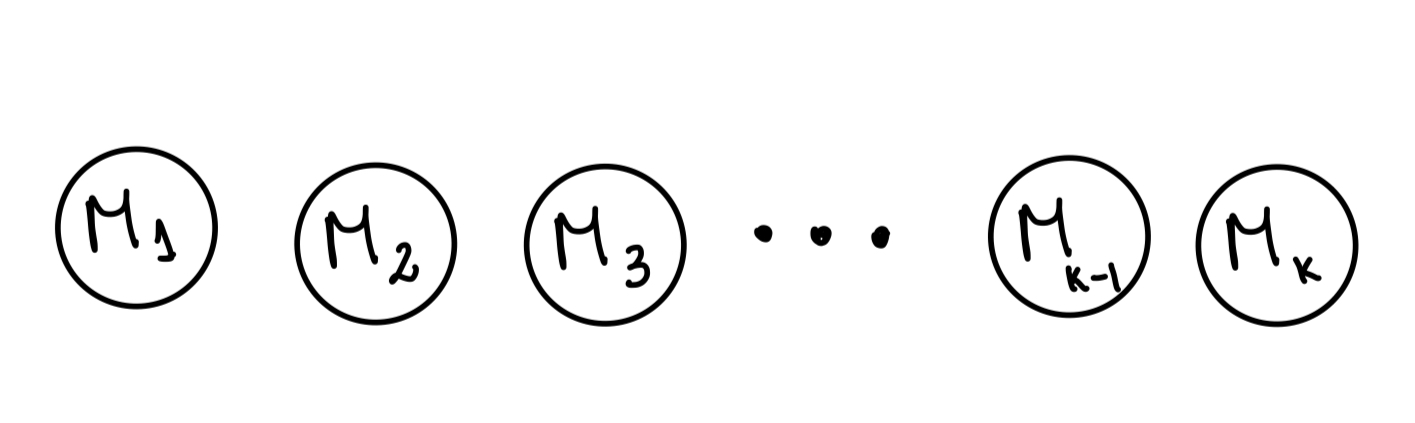
\includegraphics[width=9cm, height=3.5cm]{images/IMG_1629.jpg}

No podemos establecer quien es mayor/menor al haber k valores, ya que en la fila los valores no estan ordenados ascendente o descendentemente.

Para poder analizarlo vamos a hacer una función partida para ver cuales son nuestras opciones para cada uno:

$ValorSofiaTurno= \left\{ \begin{array}{lcc} M_{k} & si & M_{k}>M_{1} , ValorMateoTurno= \left\{ \begin{array}{lcc} M_{k-1} & si & M_{k-1}<M_{1} \\ \\ M_{1} & si & M_{k-1} > M_{1} \end{array} \right. \\ \\ M_{1} & si & M_{k} < M_{1}, ValorMateoTurno= \left\{ \begin{array}{lcc} M_{2} & si & M_{2}<M_{k} \\ \\ M_{k} & si & M_{k} < M_{2} \end{array} \right. \end{array} \right.$

En consecuencia del turno de Sofía, Mateo va a tener 2 posibilidad por cada elección.
\vskip1cm
Como podemos observar, siempre hay un patrón: Si los turnos empezaran desde el 0, Sofia siempre tiene los turnos pares
,en los cuales agarra siempre el valor de moneda más grande, y Mateo tiene los turno impares donde agarra el valor los valores más pequeños.

\vskip0.5cm

\vskip0.5cm
$valorSofiaTotal =  \sum_{k=1}^{n}M_{k}$ siendo $\left\{ \begin{array}{lcc} k=i_{inicial\_actual} & si & i_{inicial\_actual}>j_{final\_actual} \\ \\ k=j_{final\_actual} & si & i_{inicial\_actual}<j_{final\_actual} \end{array} \right.$

\vskip0.5cm
$valorMateoTotal =  \sum_{k=1}^{n}M_{k}$ siendo $\left\{ \begin{array}{lcc} k=i_{inicial\_actual} & si & i_{inicial\_actual}<j_{final\_actual} \\ \\ k=j_{final\_actual} & si & i_{inicial\_actual}>j_{final\_actual} \end{array} \right.$

\vskip0.5cm
NOTA: $i_{inicial\_actual}$ es el principio de nuestra fila de monedas por turnos, y $j_{final\_actual}$ en el final de nuestra fila por turnos 
\vskip1cm
Y para corroborar que nadie está haciendo trampa:
\vskip0.5cm
\begin{center}
    $valorTotalDeMonedas=valorSofiaTotal+valorMateoTotal$
\end{center}


